\documentclass[tikz,border=8pt]{standalone}
\usepackage{amsmath}
\usetikzlibrary{arrows.meta,positioning,fit}

\begin{document}
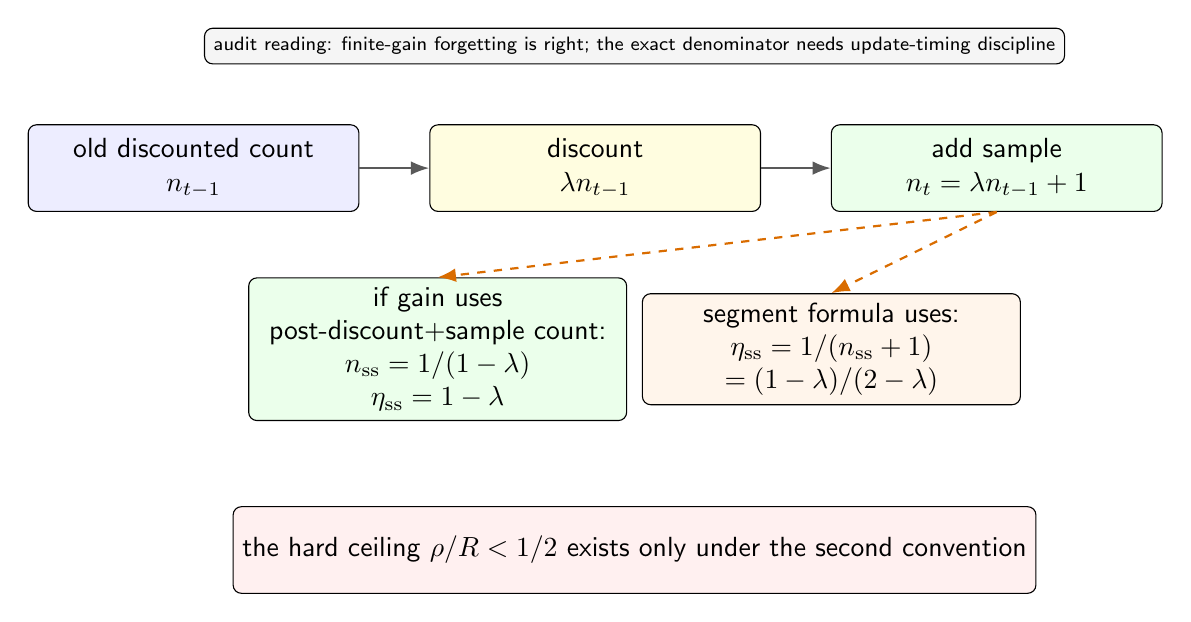
\begin{tikzpicture}[
  font=\sffamily,
  box/.style={draw, rounded corners=3pt, align=center, minimum width=42mm, minimum height=11mm, fill=white},
  note/.style={align=center, font=\sffamily\scriptsize},
  arrow/.style={-Latex, thick, draw=black!65},
  warn/.style={-Latex, thick, dashed, draw=orange!85!black}
]

\node[box, fill=blue!7] (old) at (0,1.5)
  {old discounted count\\$n_{t-1}$};
\node[box, fill=yellow!12] (disc) at (5.1,1.5)
  {discount\\$\lambda n_{t-1}$};
\node[box, fill=green!8] (add) at (10.2,1.5)
  {add sample\\$n_t=\lambda n_{t-1}+1$};

\draw[arrow] (old.east) -- (disc.west);
\draw[arrow] (disc.east) -- (add.west);

\node[box, fill=green!8, minimum width=48mm] (conv1) at (3.1,-0.8)
  {if gain uses\\post-discount+sample count:\\$n_{\rm ss}=1/(1-\lambda)$\\$\eta_{\rm ss}=1-\lambda$};
\node[box, fill=orange!8, minimum width=48mm] (conv2) at (8.1,-0.8)
  {segment formula uses:\\$\eta_{\rm ss}=1/(n_{\rm ss}+1)$\\$=(1-\lambda)/(2-\lambda)$};

\draw[warn] (add.south) -- (conv1.north);
\draw[warn] (add.south) -- (conv2.north);

\node[box, fill=red!6, minimum width=78mm] at (5.6,-3.35)
  {the hard ceiling $\rho/R<1/2$ exists only under the second convention};

\node[note, fill=gray!8, draw, rounded corners=3pt, minimum width=88mm] at (5.6,3.05)
  {audit reading: finite-gain forgetting is right; the exact denominator needs update-timing discipline};

\end{tikzpicture}
\end{document}
